\subsection{Product Prospective}
This section provides a high-level description of the Student\&Company platform, outlining its main features and functionalities throught the use of text description such as User Scenarios, and a more in-depth analysis of the system's structure through the use of Class Diagrams and State Charts.
\subsubsection{User Scenarios}
\label{subsec: user scenarios}

\begin{enumerate}
        \item \textbf{\textcolor{titleColor}{Student Sign-up}}\\
        Mario Rossi is a student that want to improve his abilities and education by doing an internship before graduating. He opens the SC root page and select “SignUp”. He provides the required personal information such as his name, surname, date of birth, an email, and a password that he will use as login credential. He also select from the list of available university the one he is attending\\
        If the email address has never been used on the site, Mario will receive an email for confirming the mail address and the registration of the account. Once the registration is confirmed by Mario, the account is created. If the email address is already in use, the platform will show an error that ask to insert a new email address.
    \item \textbf{\textcolor{titleColor}{Company Sign-up}}\\
        FastRedCar SPA, a world-leading car company, aims to launch an internship program to train final-year mechanical engineering students pursuing a Bachelor's or Master's degree. To register on the S\&C platform, the company accesses the root page and selects “Sign Up,” where they provide the required information, including the company name, headquarters address, VAT number, email address, and a password to be used as login credentials.\\
        If both the VAT number and email address have not been previously used on the platform, FastRedCar SPA will receive a confirmation email to verify the address and complete the account registration. Once the email is confirmed, the account is successfully created.\\
        However, if either the VAT number or email address is already associated with an existing account on S\&C, an error message will be displayed, indicating that the company already has a registered account on the platform.
    \item \textbf{\textcolor{titleColor}{University Sign-up}}\\
        The Technical University of Milan is a prestigious university that wants his students to complete an internship before graduating, believing this experience will enhance their skills and knowledge. The university opens the S\&C root page and selects “SignUp” where they provide the required information such as the university name, the university description, the university VAT number, the name of the university office that will manage the internship program and also an email address and a password that will be used as login credential.\\
        If both the VAT number and email address have not been previously used on the platform, the Technical University of Milan will receive an email for confirming the mail address and the registration of the account. Once the registration is confirmed, the account is created.
        However, if either the VAT number or email address is already associated with an existing account on S\&C, an error message will be displayed, indicating that the university already has a registered account on the platform.
    \item \textbf{\textcolor{titleColor}{User Login}}\\
        A platform user that has already registered an account can log in by providing the email and password used during the registration. If the email and password are correct, matching an entry in the platform DB, the user is redirected to the platform dashboard page. If the email or password are incorrect, the platform will show an error message indicating that the login credentials are wrong.
    \item \textbf{\textcolor{titleColor}{Student Load Curriculum}}\\
        Stefano is a student who has already registered an account on S\&C and wants to complete his profile by uploading his CV. From the platform's dashboard, he clicks on the “CV” button. He is then redirected to a page where he can enter his curriculum information, including his current level of education, languages he knows, technical skills, and, optionally, details about past work experience along with contact information for previous employers.
        He also adds a photo of himself, a brief description of his interests and hobbies and, as soon as he clicks on the “Submit CV” button, the platform elaborates it and try to find some matching internship based on the given information.\\
        A list of five different internships, to which Stefano has been matched, is shown to the student in the platform's recommendations page where he can decide to apply for one of them, notifying the company.
        While computing the matching, the platform also provides Stefano with some suggestions on how to improve his CV and matching probability, based on a grammar and lexical analyses and a direct comparison of Stefano's CV with other similar candidate
    \item \textbf{\textcolor{titleColor}{Company Submit an Internship Insertion}}\\
        AnanasPhone is a major tech company, specialized in the production of smartphones and tablets, that has an account on the S\&C site. The company wants to create an internship program aimed at software engineering students in the final year of their Master's degree.\\
        A Human Resource employee open the S\&C platform and select “Internships Offers” where a list of all the internship already present on S\&C are shown. Here he clicks on “Create Internship” where he provides the required information such as the internship title, the internship description, the start date and duration, the office address, a list of the required skills students need to have in order to be considered for the internship and, possibly, a list of benefits offered to the future intern. Once the internship is created, by clicking on the “Submit Internship” button, the platform will start the recommendation process with the aim to match the internship with all the students that are compatible with such opportunity, based on the given information of both parties.\\
        %I propose to leave this as "singular" because each time a intership offer is created some suggiestions are given but only for that offer
        The platform will also provide AnanasPhone with some suggestions on how to improve the internship description, and matching probability, based on a grammar and lexical analyses and a direct comparing of AnanasPhone's Internship proposal with other similar companies.
    \item \textbf{\textcolor{titleColor}{Company create a structured interview to submit to possible candidate}}\\
        MacroHard is a world-leading tech company, known for creating its secure and reliable operating system, “Door”. The company has an account on the S\&C platform and has already set up an internship program for software engineering students pursuing a Master’s degree. The company wants to create a structured interview to evaluate the technical skills and motivation of the students who apply for the internship.\\
        MacroHard opens the platform dashboard and, on the page displaying the lists of matched students, clicks on the “Create Interview” button. This option allows the company to create structured interviews that will be submitted to candidates. 
        MacroHard can create multiple interviews for the same internship, allowing to submit them to different students based on factors such as the student’s CV, method of application (matched or spontaneous), or other criteria. \\
        For this internship, MacroHard has created two types of interviews: one for matched students to assess their technical skills, and another for spontaneous applicants, which evaluates not only technical skills but also the student's motivation.
    \item \textbf{\textcolor{titleColor}{Student accepts a matched internship}}\\
        Sara is an economic major student that has already uploaded her CV on the S\&C platform, and she is looking for an internship. She has received a notification and, by clicking on it, she sees that a new internship is available for her.\\
        Sara reads the internship information, and she decides to accept it. A notification is then sent to the company that created the internship informing them of Sara's acceptance of the match. If the company also accepts the match, the platform requires the company to initiate the selection process by creating or assigning a structured interview to Sara, who will be notified about it.
        To both parties, feedback is requested by the platform to improve the Recommendation Process by asking both to rate the matching generated by S\&C  
    \item \textbf{\textcolor{titleColor}{Student manually applies for an internship}}\\
        Marco is a chemistry student that has already uploaded his CV on the S\&C platform and is looking for an internship. Unfortunately, the matching internships provided by the platform do not fully satisfy his needs, and he decides to proactively search for another one.\\
        He opens the platform's dashboard page and click on the “Spontaneous Application” button. Here he can see all the internships that are available on the platform, and he can filter them by field of study, required skills, location and other parameters.
        He finds an internship that is not in the matching list provided by the platform, but that is perfect for him, so he clicks on the “Apply” button.\\
        The platform notifies the company that Marco has applied for the internship and will inform the student the company will start the application process by sending him an interview. There is no need for Marco to accept the interview, as a spontaneous application is considered as an implicit acceptance of the match by the student.
    \item \textbf{\textcolor{titleColor}{Student see his application  interview status}}\\
        Stefano is a student who has applied for various internships through the S\&C platform. He has submitted applications, both by matching with companies through the platform's automated feature, and by manually applying. He is already in a selection phase with some of them, and he is currently waiting for updates from the different companies.\\
        When Stefano logs into the platform, he navigates to “Interviews”. In this section, he can view the status of each of his applications by clicking on each one of them. This includes whether the company has assigned him an interview, whether his interview has been reviewed, and whether he has been accepted or rejected for the position. In the same section, he can also see if the platform is running the recommendation process, matching his profile with all the other possible internship offers.
    \item \textbf{\textcolor{titleColor}{Company see the status of the selection process}}\\
        CosmoX, a renowned private space company that is specialized in the reuse of rocket, has created an internship on the S\&C platform for aspirants Aerospace engineers. It has received multiple manual applications from different students and has been match numerous time. The company has already accepted all worthy manual applications and matches and has assigned structured interviews to everyone. CosmoX is now waiting for the students to complete the interviews.\\
        When a CosmoX employee logs into the platform, he can navigate to the “Interview” section. In this section, he can view the status of each interview and the status of each student, such as: “SENT” if the student has received the interview but not opened yet, “COMPLETED” if the student has completed the interview and “REVIEWED” if the company has started the review process of the interview.
    \item \textbf{\textcolor{titleColor}{Student refuse/accept an internship}}\\
        Paula is an Art Major that has been matched by S\&C with different museums and private art galleries in the city of Florence. She happily accepted all the matches and completed the interviews with all the companies. She did not expect to pass all the interviews, and now she has to choose between the different offers.\\
        Paula open the platform and navigate to the “Interview” section, where she can see all of her interview and the status of each one. To refuse an internship position after successfully passing the interview, Paula clicks on it and then clicks on the “Refuse” button, and the platform will notify the company about her the decision. By doing the same process, but clicking on the “Accept” button, the platform will notify the company that Paula has accepted the internship and will and block any other interview process informing the respective companies.\\ 
        By navigating to the “Interview” section, any company can see, between the different possible state of an application, if the internship of a particular student has been accepted or refused.
    \item \textbf{\textcolor{titleColor}{Company publishes a complaint about a student}}\\
        PlaneHearts is a company famous for its innovative and multi-platform IDE for the development of mobile applications. The company has created an internship on the S\&C platform for software engineering students and selected Giovanni, a computer science student, for the internship. However, after the internship started, employees at PlaneHearts noticed that Giovanni was not performing as expected, did not have the required skills, and was not motivated to learn. The company decided to publish a complaint about Giovanni on the platform to inform the student's university.\\
        For publish the complaint, the person managing PlaneHearts account on S\&C, logs into the platform and navigates to the “Complaints” section. Here, he can view all the complaints they have published and can create a new complaint by providing the student's name, the internship title, and describing the problem that has arisen. Once the complaint is submitted, the platform will notify Giovanni and his university.
    \item \textbf{\textcolor{titleColor}{Student responds to a complaint}}\\
        Giovanni has received a notification from the S\&C platform that a complaint has been published about him by PlaneHearts, the company where he is currently doing an internship. The complaint states that Giovanni is not performing as expected, does not have the required skills, and is not motivated to learn during this experience.\\
        The Student will have the opportunity to respond to the complaint and provide his version of the events by navigating to the “Complaints” section of the platform. Here, he can view all the complaints published about him and can respond to each one by providing a description of the situation from his perspective.
    \item \textbf{\textcolor{titleColor}{University handles a complaint}}\\
        The University of Rome, a prestigious university that has students enrolled in the S\&C platform, has received a complaint about one of their students. The carrier advisor at the university opens the S\&C platform and navigate to the “Complaints” section. Here, he can view all the complaints published about his students and can handle each one by reviewing the complaint, contacting the student and the company involved, and taking appropriate actions to resolve the issue.
        In this particular case, the advisor and the university have decided to interrupt the internship of the student to protect the student and the company from further issues. The university do so by clicking on the “Interrupt Internship” button in the complaint page. The platform will notify the student and the company about the interruption of the internship and will close the complaint.
\end{enumerate}
\subsubsection{Class Diagrams}
The following UML class diagram describes the domain of our interest with the entities involved in it and the main relations between them. It includes the main attributes and a limited set of methods that represent the core functionalities of the system. These entities capture the essence of the platform's domain.
\begin{figure}[H]
    \centering
    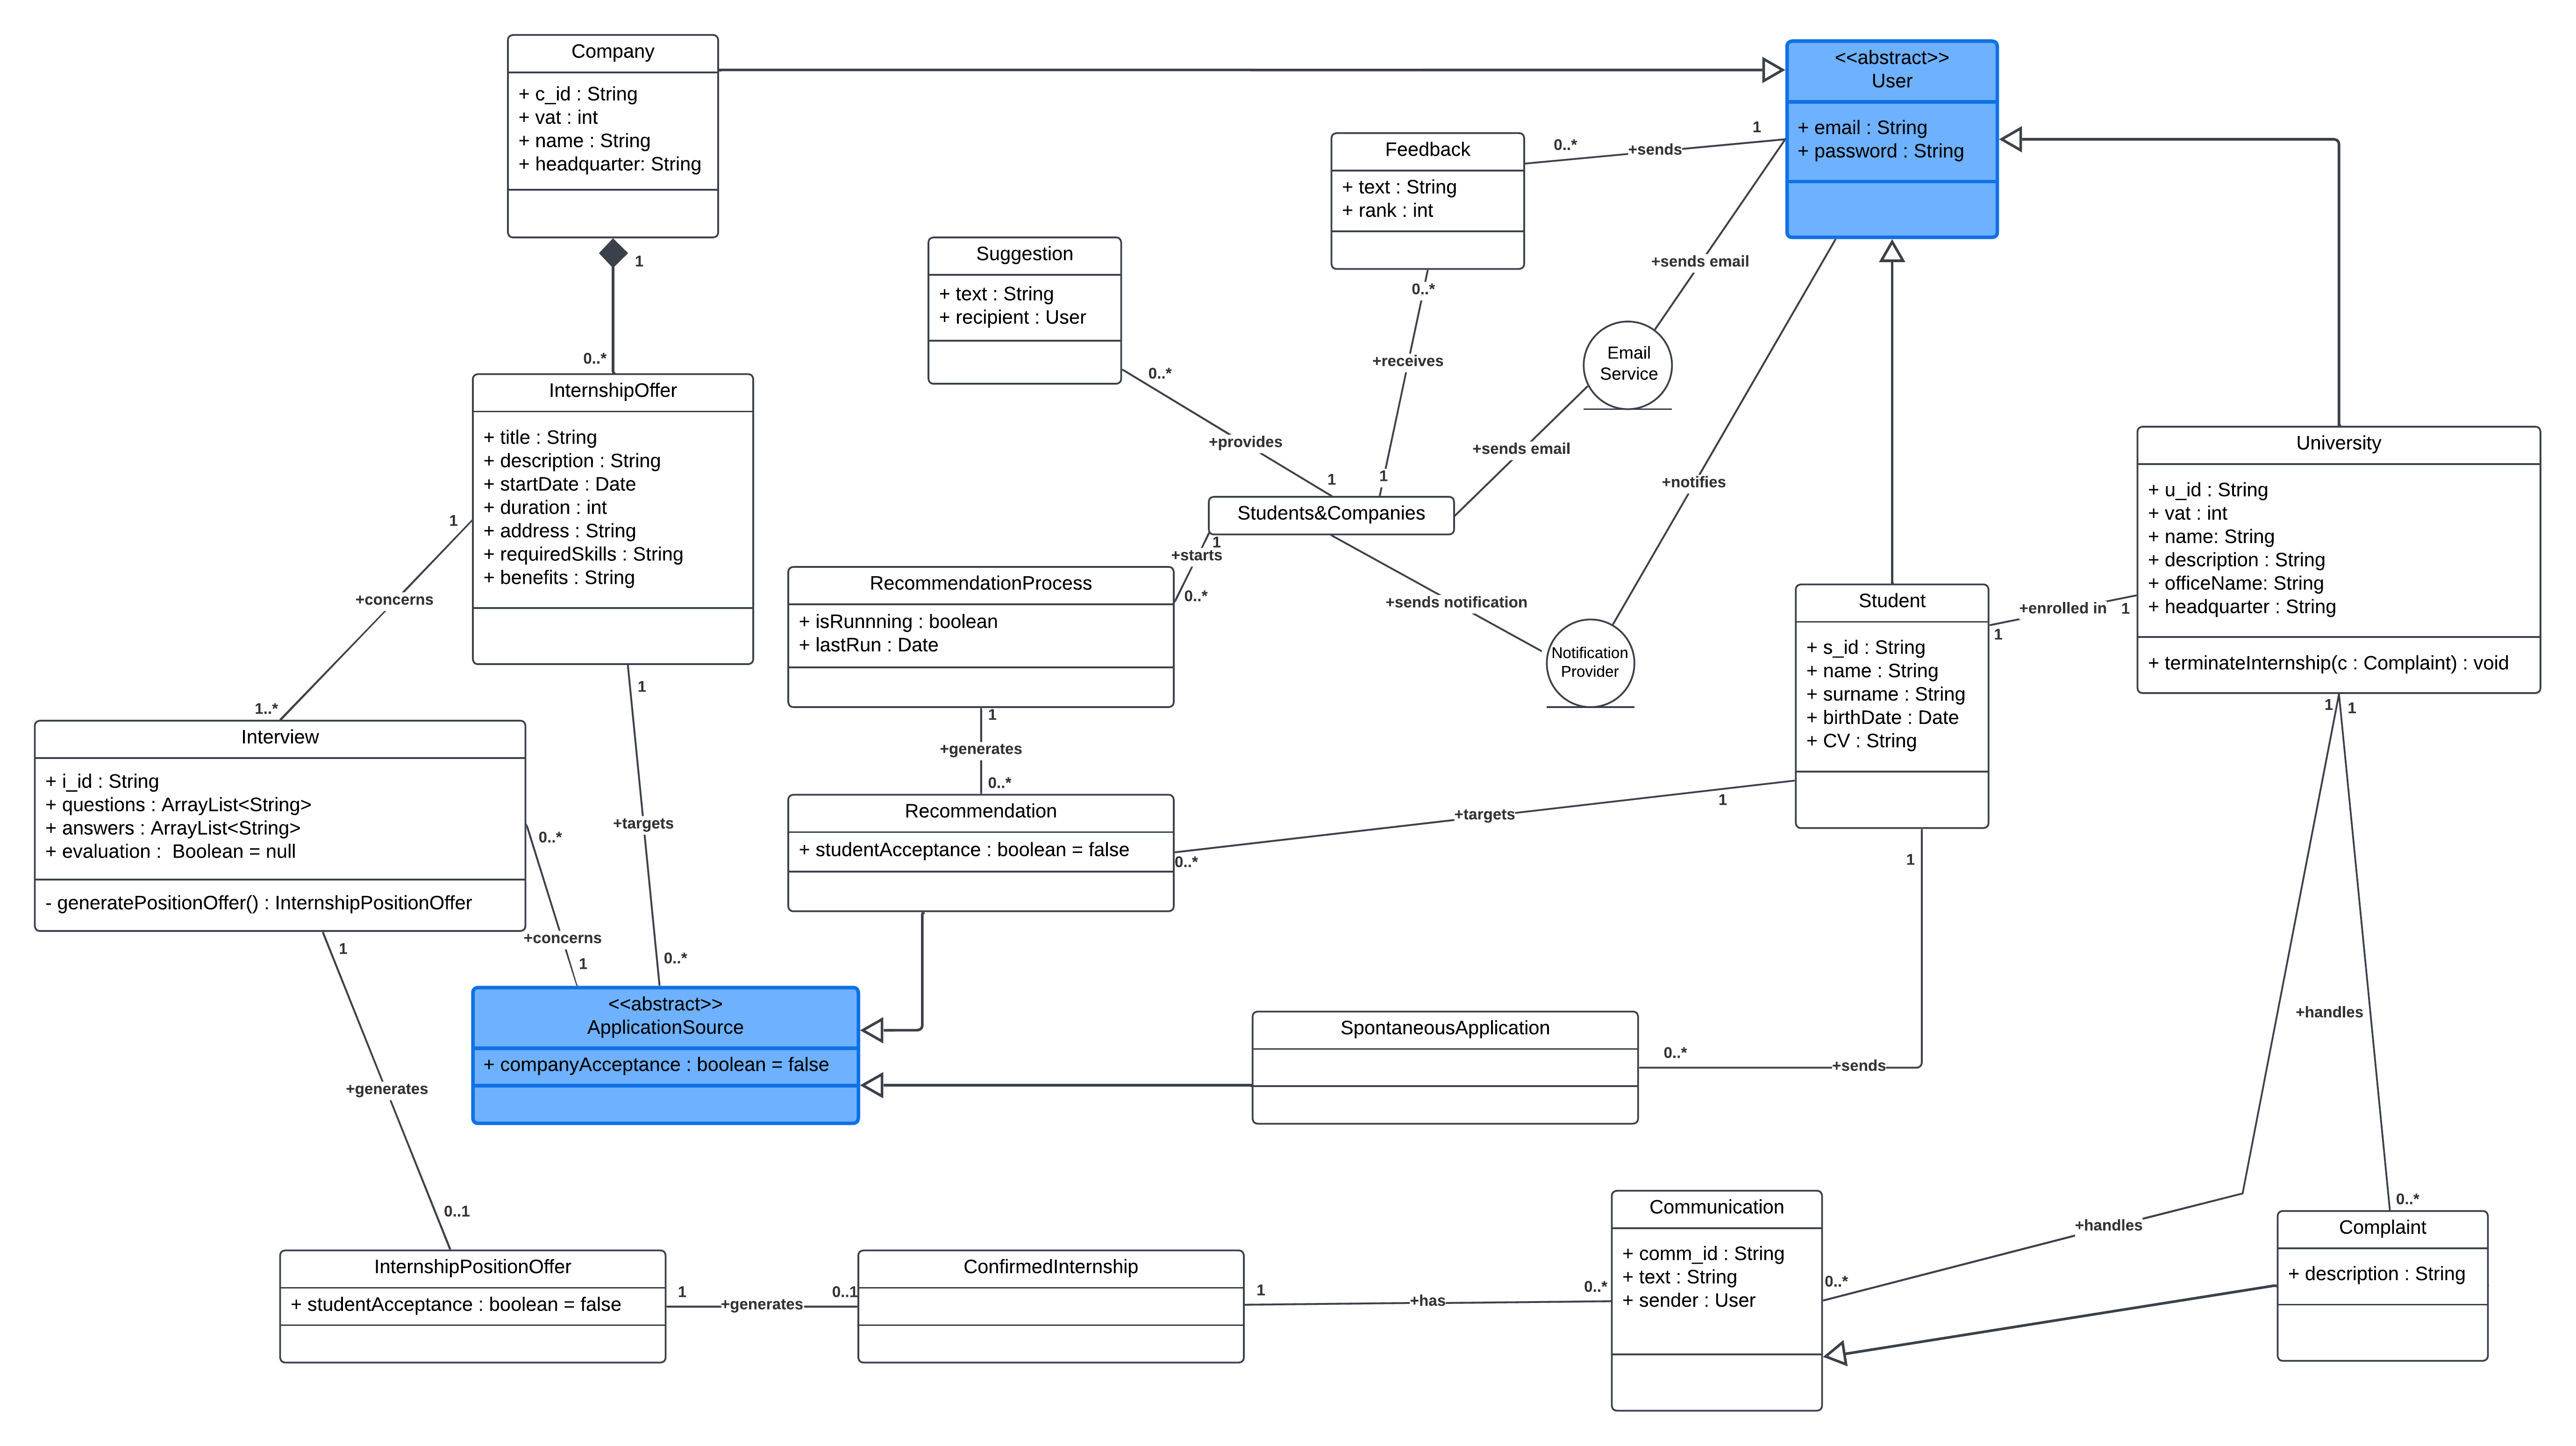
\includegraphics[width=\linewidth]{Latex/Images/ClassDiagram2.1.png}
    \caption{Class Diagram}
    \label{fig:ClassDiagram}
\end{figure}
To clarify the methods signatures:
\begin{itemize}
    \item Interview: \verb|generatePositionOffer(): InternshipPositionOffer| \\generates the \verb|InternshipPositionOffer| if the company wants to provide the student who passed an interview with an Internship Position Offer. 
    \item University: \verb|terminateinternship(c: Complaint): void| \\allow the University to terminate an Internship through a Complaint.
\end{itemize}
Other methods have been omitted for semplicity, as the relations are sufficient to understand the domain. 
\clearpage
\subsubsection{State Charts}
The following section presents a series of state diagrams illustrating the progression of the main phases of the Student\&Company platform. These diagrams include representations of the Recommendation Process and its Spontaneous Application variant, the Interview Process that may result in an Internship Position Offer, and finally, a Selection Process diagram that highlights the relationship between the latter two processes.
These diagrams represent the possible states that the object Interview can be in, without detailing all possible outcomes explicitly. For example, the case of the interview accepted or rejected are represented into a single state, InternshipEnded, without loss of generality.
\newline\newline
\noindent\textbf{\color{titleColor}Recommendation Process}\\
\begin{figure}[ht]
    \centering
    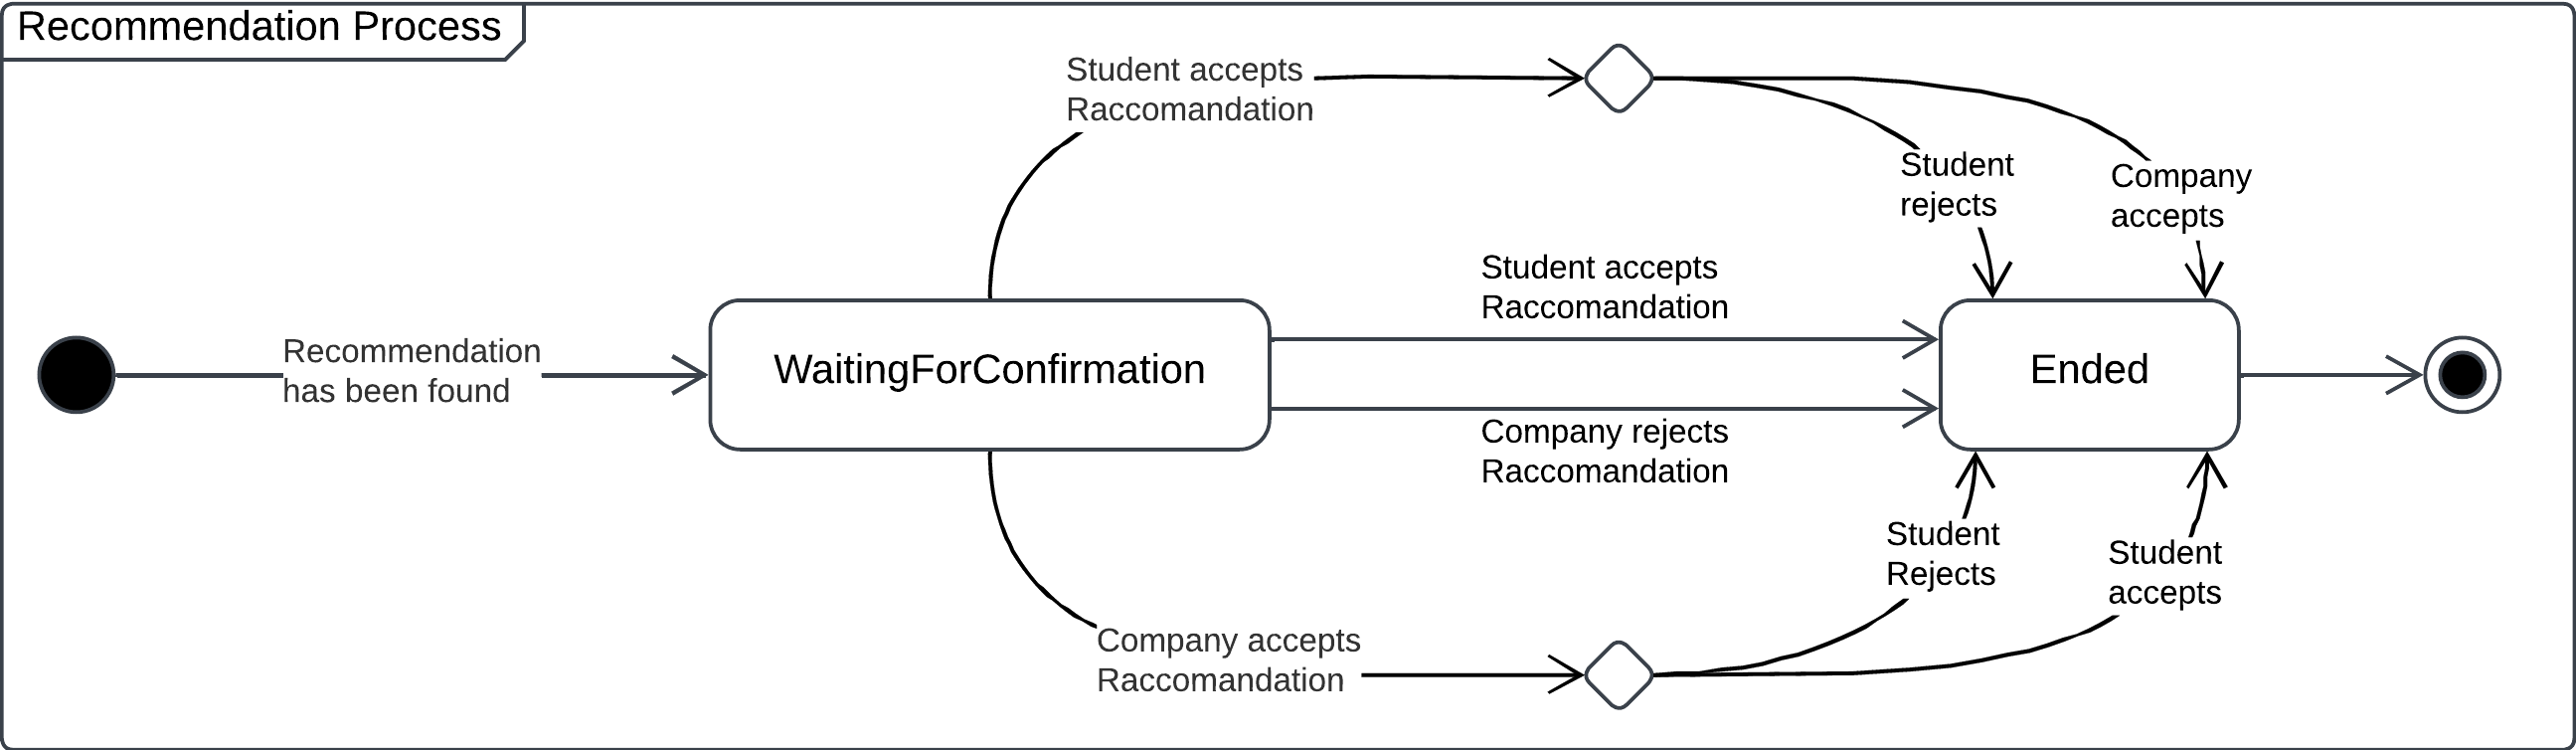
\includegraphics[width=1 \textwidth]{Latex/Images/RecommendationStateChart.png}
    \caption{Recommendation State Chart}
    \label{fig:RecommendationProcess}
\end{figure}
\begin{itemize}
    \item The Recommendation Process is the core of the Student\&Company platform. It is the process that matches Students with Internships based on the Student's CV and the Internship's requirements. It is initiated by the platform when it detects a potential Match. The process then evolves to a "ToBeAccepted" state, where the system waits for the Student and the Company to accept the Match. If one of the two parties rejects the Match, the process is terminated. If both parties accept the Match, an Interview is initiated, and the process is terminated.
\end{itemize}

\noindent\textbf{\color{titleColor}Spontaneous Application Process}\\
\begin{figure}[ht]
    \centering
    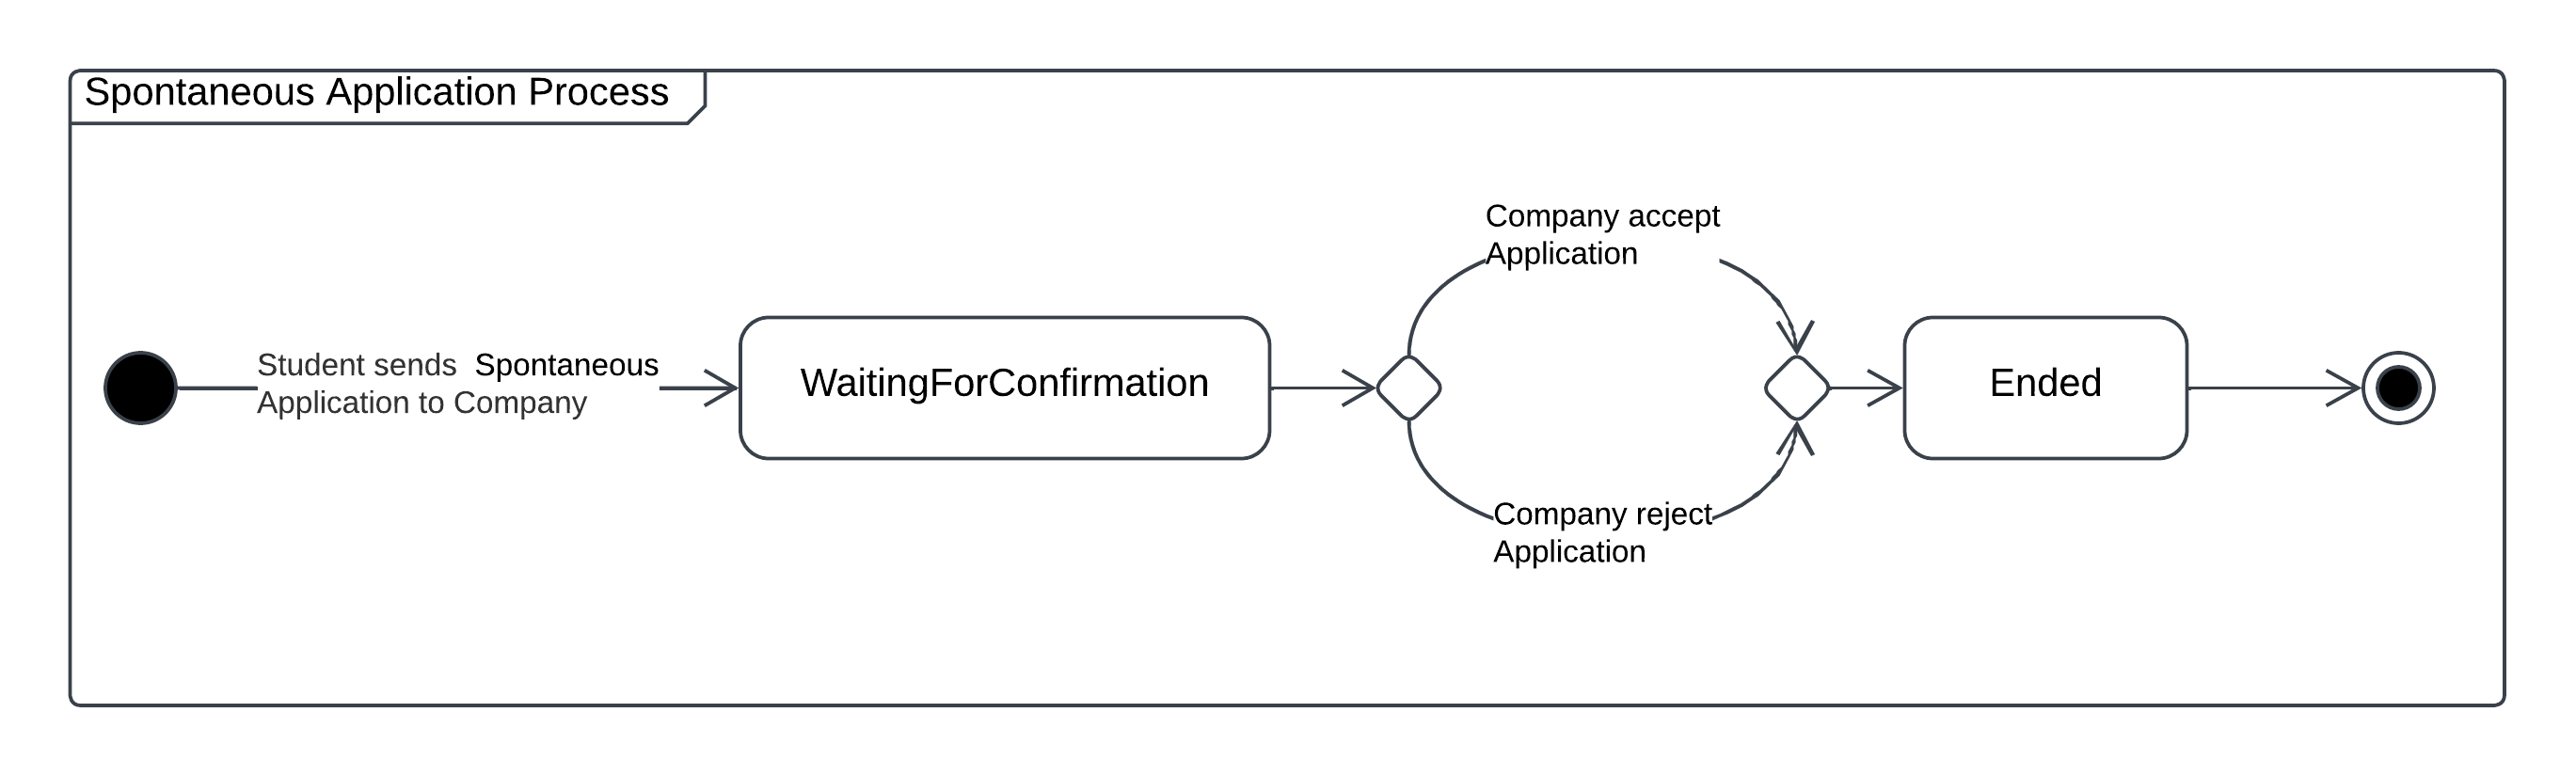
\includegraphics[width=1 \textwidth]{Latex/Images/SpontaneousApplicationStateChart.png}
    \caption{Spontaneous Application State Chart}
    \label{fig:SpontaneousApplication}
\end{figure}
\begin{itemize}
    \item Unlike the Recommendation Process, the Spontaneous Application process is initiated by the Student. When a Student submits a Spontaneous Application for an Internship, the process evolves to a "ToBeAccepted" state, where the system waits for the Company to accept the Application. If the Company rejects the Application, the process is terminated. If the Company accepts the Application, an Interview Process is initiated, and the process is terminated.
\end{itemize} 
\clearpage
\noindent\textbf{\color{titleColor}Interview Process}\\
\begin{figure}[H]
    \centering
    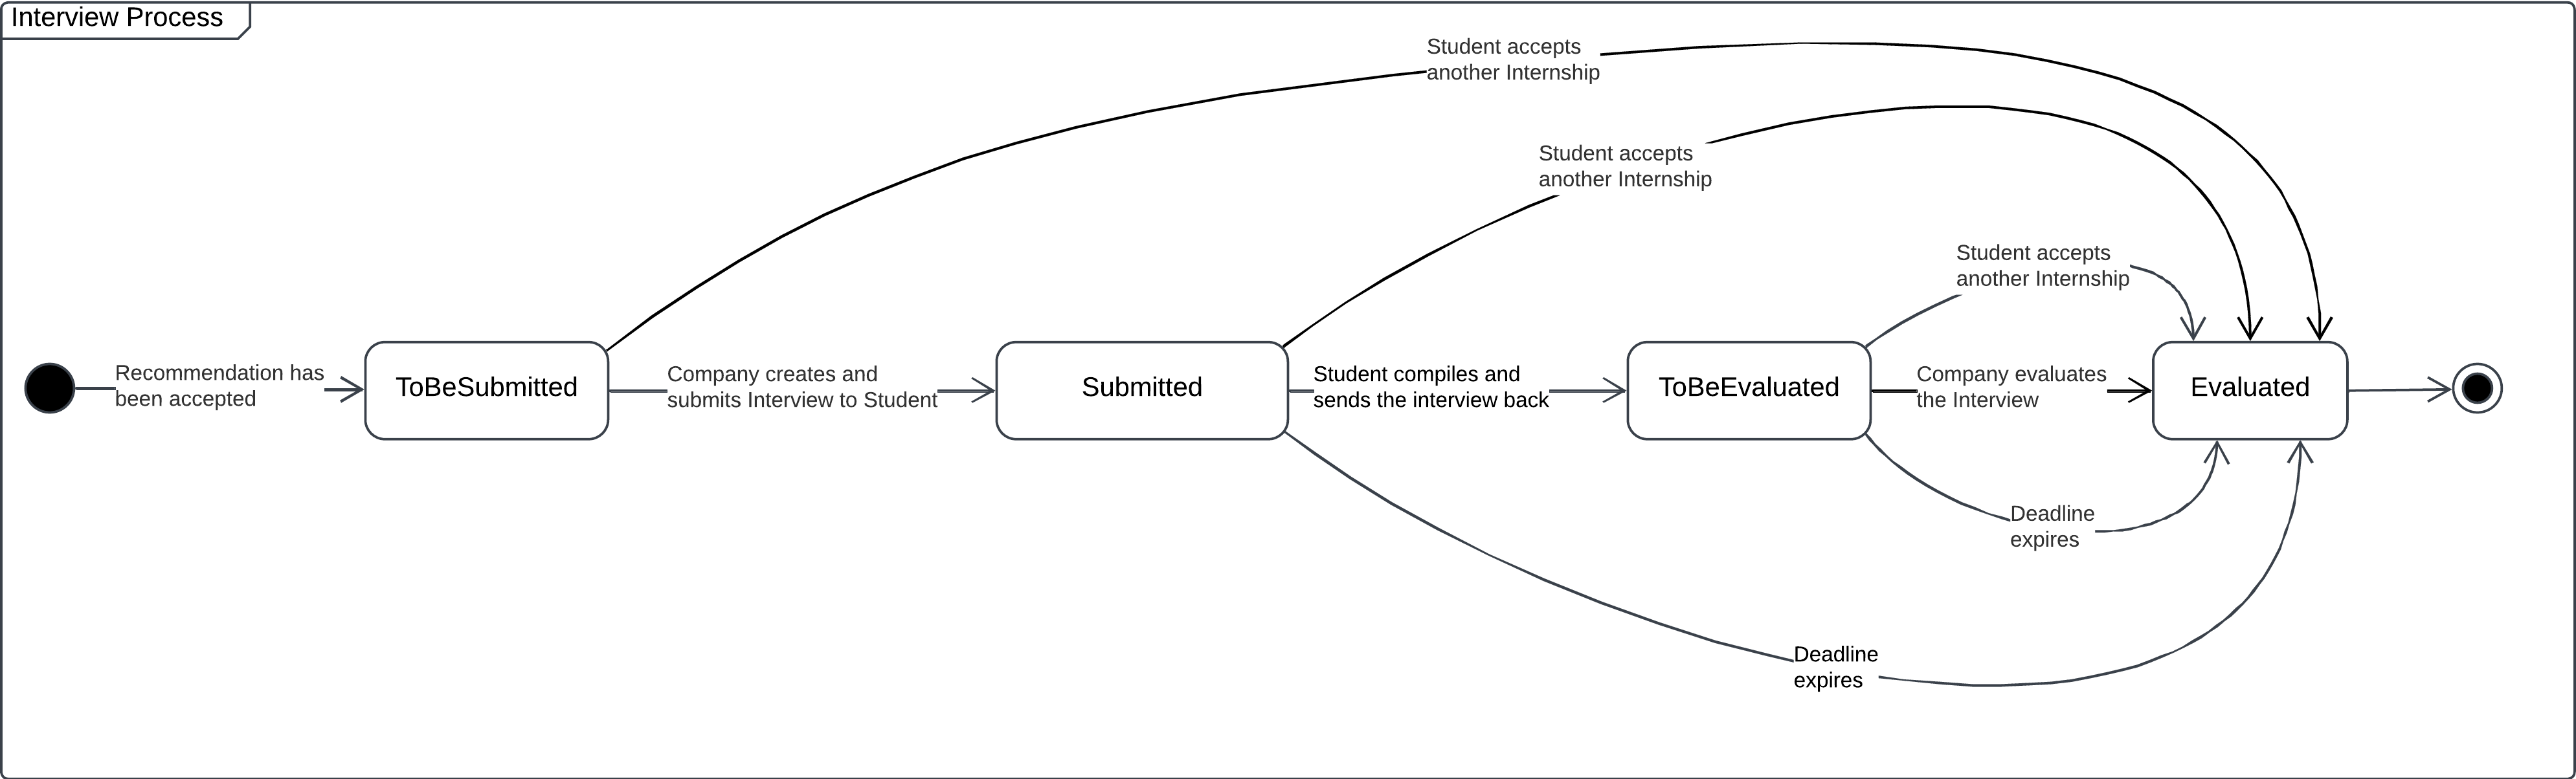
\includegraphics[width=1 \textwidth]{Latex/Images/InterviewProcessStateChart.png}
    \caption{Interview State Chart}
    \label{fig:InterviewProcess}
\end{figure}
\begin{itemize}
    \item The Interview Process is initiated when a Match is accepted by both the Student and the Company, or when the Company accepts a Spontaneous Application. The process starts in the “ToBeSubmitted” state, where the Company is asked to create and submit an Interview. Here, the Company is required to specify a deadline for the Interview. The Interview process evolves into the “Submitted” state once the Company sends the Interview to the Student, who answers the questions and submits the Interview. If the Student fails to submit the answers within the deadline, he will be considered rejected, and the process is progressed to an "Evaluated" state and terminates. Otherwise, after the Interview has been sent back by the student, the process evolves to a “ToBeEvaluated” state. In this state, the Company can manually evaluate the Student's answers and mark the interview as accepted or rejected. In case the Student has been rejected, he will be notified of the outcome, and the process is terminated. Otherwise, if the Student has been accepted, an Internship Position Offer process started and the Interview Process is terminated. If anywhere in the process, the Student accepts another Internship, the process terminates and the Student will be considered rejected.
\end{itemize}

\noindent\textbf{\color{titleColor}Internship Position Offer process}\\
\begin{figure}[H]
    \centering
    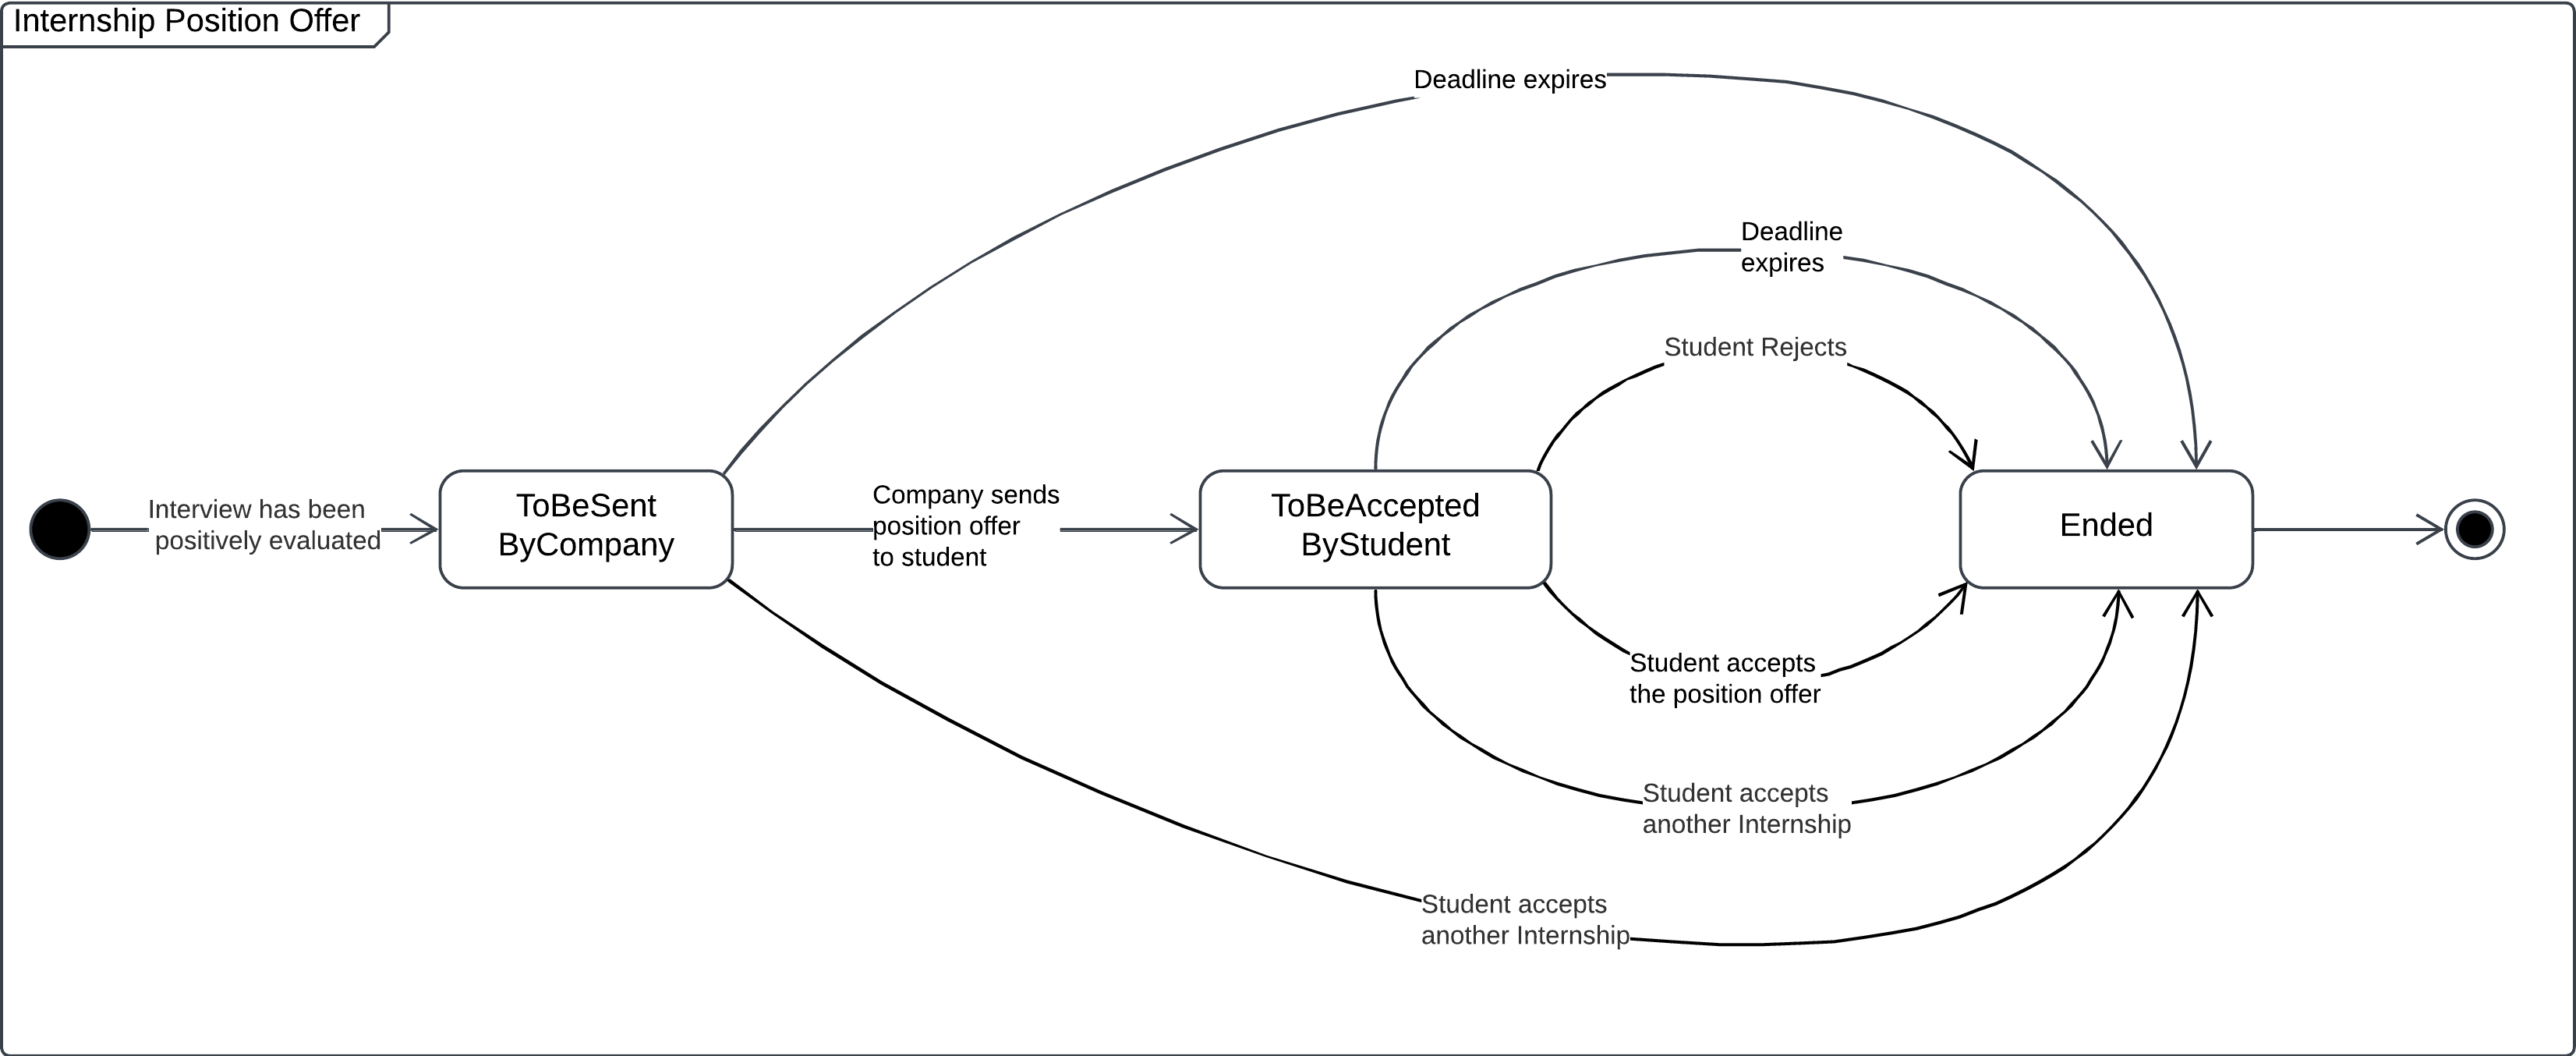
\includegraphics[width=1 \textwidth]{Latex/Images/InternshipPositionOfferStateChart.png}    
    \caption{Internship Position Offer State Chart}
    \label{fig:InternshipPositionOffer}
\end{figure}
\begin{itemize}
    \item The Internship Position Offer process begins when a student successfully completes the Interview Process. Initially, the process enters the “ToBeSentByCompany” state.
    This state allows companies to evaluate and select the most suitable candidates when more students than required have passed the interview.
    If the company rejects the student or the deadline expires, the process concludes, and the student will be considered rejected.
    If the company accepts the student, the process transitions to the “ToBeAcceptedByStudent” state, where the student decides to either accept or reject the offer.
    If the student rejects the offer or lets the deadline expire, the process concludes, and the student will be considered rejected.
    If the student accepts the offer, the process concludes, and all the student’s other ongoing interviews are terminated with the student being marked as rejected in those interviews.
    If anywhere in the process, the Student accepts another Internship, the process is terminated and the Student will be considered rejected.
\end{itemize}

\noindent\textbf{\color{titleColor}Selection Process}\\
\begin{figure}[H]
    \centering
    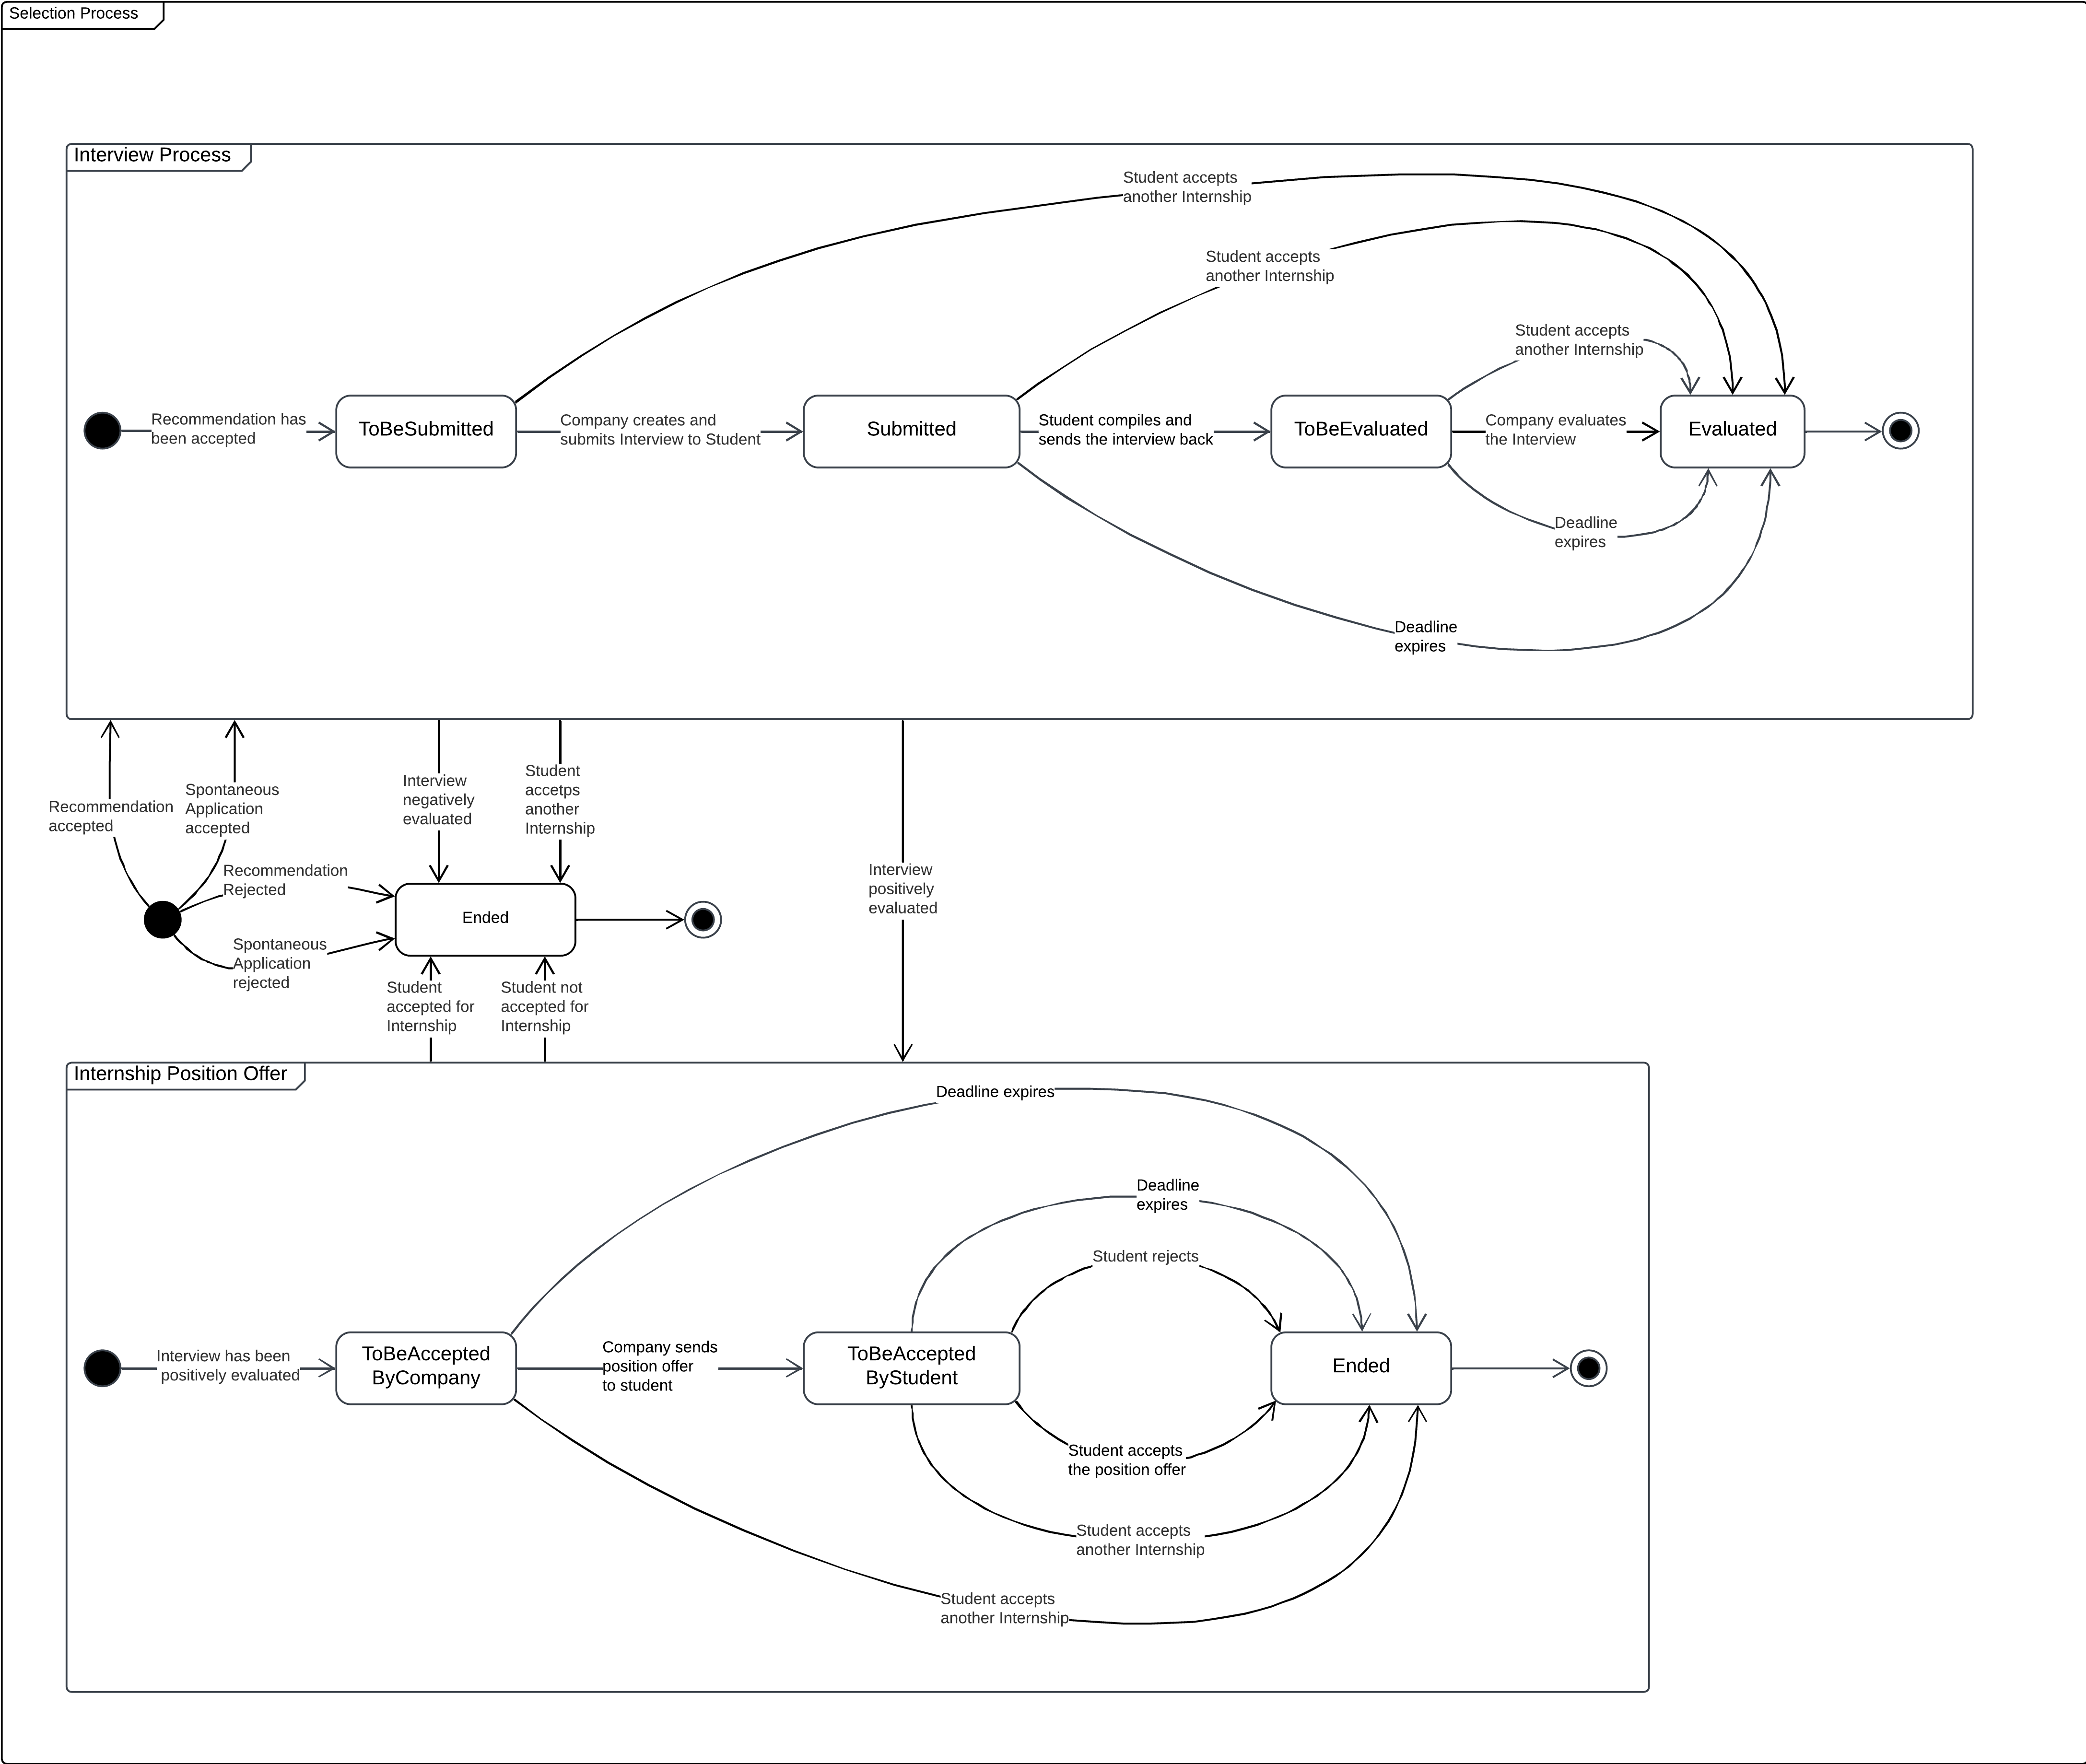
\includegraphics[width=1 \textwidth]{Latex/Images/SelectionProcessStateChart.png}
    \caption{Selection Process State Chart}
    \label{fig:SelectionProcess}
\end{figure}
\begin{itemize}
    \item The Selection Process diagram illustrates the relationship between the Interview Process and the Internship Position Offer Process.
    The Selection Process terminates if the Match is rejected, if the Student is rejected during the Interview Process or the Internship Position Offer Process, or if the Student accepts another Internship.
    If the Student is accepted during the Interview Process, the process transitions to the Internship Position Offer Process.
    If the Student accepts the Internship Position Offer, the process also concludes.
\end{itemize}
\clearpage
\subsection{Product Functions}
This section outlines the essential functionalities and detailed requirements of the platform, structured to support the key objectives defined in the scope of the product.
\begin{enumerate}
    \item \textbf{\color{titleColor}User Management}: The platform allows Students, Companies, and Universities to register and log in. It also provides Students with the ability to upload and modify their CVs, and Companies with the ability to view and manage their Internships.
    \item \textbf{\color{titleColor}Internship Creation and Management}: Companies can create, publish, and manage Internship offers on the platform. They define details such as job description, requirements, deadlines, and benefits. Companies also have the ability to terminate Internship offers when they are no longer available.
    \item \textbf{\color{titleColor}Student Application Process}: Students can browse available Internships and apply to Internships either through automatic matching or by submitting Spontaneous Applications. They can also track the status of their Applications throughout the process.
    \item \textbf{\color{titleColor}Automated Recommendations}: The platform matches Students with suitable Internships based on their CVs and the specific requirements set by Companies. Once a match is found, both Students and Companies are notified, and they can accept or decline the Recommendation.
    \item \textbf{\color{titleColor}Interview Management}: Companies can create and assign Interviews to Students, which include closed and open questions to assess their suitability for an Internship. Both Students and Companies can track the Interview progress, and Companies can evaluate Student responses. Companies can also select among students who have passed the interview those to whom they will propose an Internship Position Offer.
    \item \textbf{\color{titleColor}Feedback and Suggestions for Improvement}: The platform collects Feedback from Students and Companies to improve the Recommendation Process. It also provides Suggestions to Students on how to enhance their CVs and to Companies on how to improve their Internship descriptions.
    \item \textbf{\color{titleColor}Complaint Management}: Students and Companies can publish Complaints about Ongoing Internships, which are then handled by Universities. Universities can monitor Complaints and interrupt Ongoing Internships if necessary.
    \item \textbf{\color{titleColor}Notification System}: Notifications are sent to Students, Companies, and Universities when relevant events occur, such as new Internships, matched Recommendations, Interview assignments,  Internship Position Offers, Sign-up confirmation, Complains or Communications.
\end{enumerate}

\subsubsection{Requirements}
\begin{enumerate}[label={\color{titleColor}[R\arabic*]}]
    % Login
    \item The platform shall allow any unregistered students to register by providing personal information and selecting their University.
    \item The platform shall allow any companies to register by providing company information.
    \item The platform shall allow any universities to register by providing university information.
    \item The platform shall allow Users to log in using their email and password.
    \item The platform shall send notifications to Users when relevant events occur.
    
    % Application advertisement and Applications
    \item The platform shall allow Companies to create and publish Internship offers specifying details.
    \item The platform shall allow Companies to terminate their Internship offers at their own discretion.
    \item The platform shall provide Students with Matches automatically obtained by the Recommendation Process.
    \item The platform shall allow Students to view and navigate all available Internships.
    \item The platform shall enable Students to submit Spontaneous Applications to Internships they choose.
    \item The platform shall allow Students to submit their CV.
    \item The platform shall allow Students to modify their CV.
    \item The platform shall allow Students to monitor the status of their Spontaneous Applications.
    \item The platform shall allow Students to monitor the status of their Recommendation.
    
    % Recommendation system
    \item The platform shall display to Students all the Internships found by the Recommendation Process.
    \item The platform shall display to Companies all the CVs of Matched Students obtained by the Recommendation Process.
    \item The platform shall allow Students and Companies to accept a Recommendation.
    \item The platform shall allow Companies to accept a Spontaneous Application.
    \item The platform shall start a Selection Process only if both the Company and the Student have accepted the Recommendation.
    \item The platform shall start a Selection Process only if the Company has accepted the Spontaneous Application.
    
    % Selection and Interview Management
    \item The platform shall allow Companies to create Interviews.
    \item The platform shall allow Companies to submit Interviews to Students they have initiated a Selection Process with.
    \item The platform shall allow Students to answer Interview questions and submit them.
    \item The platform shall allow Companies to manually evaluate Interview submissions.
    \item The platform shall allow Students and Companies to monitor the status of their Interviews.
    \item The platform shall enable Companies to complete the Interview process by submitting the final outcome to each candidate.

    %Internship Position Offer
    \item The platform shall enable Companies to send an Internship Position Offer to a Student only if he previously passed the relative Interview.
    \item The platform shall enable Students to accept or reject an Internship Position Offer sent by a Company only if he previously passed the relative Interview.
    
    % Feedback and Suggestions for Improvements
    \item The platform shall collect Feedback from both Students and Companies regarding the Recommendation Process.
    \item The platform shall provide Suggestions to Students on improving their CVs.
    \item The platform shall provide Suggestions to Companies on improving Internship descriptions.
    
    % Universities Oversight and Complaint Management
    \item The platform shall allow registered Universities to access and monitor Internship Communications related to their Students.
    \item The platform shall provide a dedicated space for Students and Companies to exchange Communications about the current status of an Ongoing Internship.
    \item The platform shall allow registered Universities to handle Complaints and to interrupt an Internship at their own discretion.
\end{enumerate}


\subsection{User Characteristics}
Student\&Company is designed to be used by three main types of Users: Students, Companies, and Universities. Each User has a specific roles and can perform different action on the platform as described below:
\begin{itemize}
  \item \textbf{Students}: \\
    Students are individuals currently enrolled in a University (which must be registered on the Platform) who are looking for Internship opportunities to enhance their education and their curriculum. \\
    They can register on the platform, upload their CVs, and apply for Internships either through the Recommendation Process or by submitting a Spontaneous Applications to a Interview Offer to which they are particularly interested. Students can also monitor the status of their Applications, Interviews, and Internship Position Offers thought dedicated section on the platform and can, eventually, report problems encountered during an Ongoing Internship to their University by creating a Complaint.\\
    The platform also provides Students with Suggestions on how to improve their CVs and matching probability based on a grammar and lexical analyses and a direct comparison of the Student's CV with another similar candidate. The Student can also improve the platform by providing Feedback on the Recommendation Process once a Confirmed Match is found.
  \item \textbf{Companies}:\\
    Companies are entities that are looking for interns to train and educate in their field of expertise. Each company account is created by a representative of the Company, usually a Human Resource employee or a manager that is in charge of the internship program. \\
    Companies can register on the platform and create, publish, manage and delete different Internship Offers at the same time. They can also view and manage the CVs of Students that have been matched or have sent a Spontaneous Application to such offers, and create and submit Interviews to evaluate them. If a Student passes the Interview, the Company can send an Internship Position Offer to him while monitoring other Interviews and Internship Position Offers and, moreover, each Company can report problems encountered during an Ongoing Internship by creating Complaints.\\
    The platform also provides Companies with Suggestions on how to improve their Internship descriptions and matching probability based on a grammar and lexical analysis and a direct comparison of the Company's Internship Offer with other similar companies. They can also help improve the platform by providing Feedback on the Recommendation Process once a Confirmed Match is found.
  \item \textbf{Universities}:\\
    Universities are institutions that are looking to provide their Students with Internship opportunities to enhance their education and curriculum. Each university account is created by a representative of the University, usually a carrier advisor or a professor that is in charge of the internship program.\\
    Universities can register on the platform and monitor their Students by receiving Communication both from Student and Companies. Such Communication can be about the acceptance of an Internship Position Offer by a Student or some problem encountered during an Ongoing Internship reported by a party trough a Complaint. \\
    The University can handle such Complaints and, eventually, interrupt an Ongoing Internship if no solution to the problem is found to prevent further issues.
\end{itemize}
While Student\&Company is not specifically designed to accommodate users with special needs, the platform implements several basic accessibility features to improve usability for all users. These include different display modes such as dark mode, screen-reader compatible layouts and easily readable fonts.
The web interface try to follows WCAG 2.1 Level A guidelines for basic accessibility compliance. However, users requiring specialized assistive technologies may need to rely on their own tools and software to interact with the platform optimally.

\subsection{Assumptions, dependencies, and constraints}

\subsubsection{Domain Assumption}
This section outlines the basic assumptions about the environment and behavior of entities that interact with the system. These assumptions simplify the design and implementation by defining expectations about Students, Companies, Universities, and the platform, ensuring the system operates effectively within its intended context.
\begin{enumerate}[label={\color{titleColor}[D\arabic*]}]
    \item Students and Companies provide the Platform with correct and truthful information.
    \item Companies remove published Internships if they are no longer available.
    \item The Email Provider and Notification Manager services are reliable, and the Users visualize every notification
    \item Students, Companies, and Universities have a working internet connection.
    \item Universities interrupt an Ongoing Internship only if no solution is found to the Complaints.
\end{enumerate}

\subsubsection{Dependencies}
The platform depends on only two external actors: the Notification Provider and the Email Service.
The former is responsible for correctly handling notifications to ensure they are sent to Users. 
The latter is responsible for sending emails, mainly for users' email verification. For more details, see section \ref{subsec:SWInteface}